\section{Klassische Enterprise-Architektur}

%%%%%%%%%%%%%%%%%%%%%%%%%% Microkernel Architecture %%%%%%%%%%%%%%%%%%%%%%%%%%%

\begin{frame}{Monolith Architecture}
    \begin{itemize}
        \item Traditionelle Architektur-Muster für die Entwicklung neuer Anwendungen
        \item Eng gekoppelte Komponenten mit gegenseitigen Abhängigkeiten
        \item Gesamte Funktionalität ist in einem einzigen Anwendung
        \item Bietet Vorteile für kleinere Anwendungen, insbesondere bei der Integration von 
          querschnittlichen Aspekten wie Logging und Sicherheitsmechanismen.
        \item Probleme treten vor allem dann auf, wenn die Codebasis wächst und an Komplexität zunimmt.
      \end{itemize}
\end{frame}

\begin{frame}{Monolith Architecture: Struktur}
    \begin{figure}[!h]
        \centering
        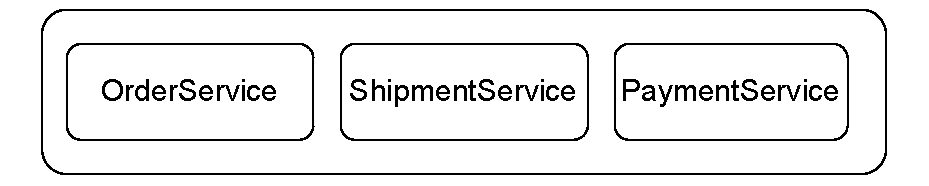
\includegraphics[scale=0.55]{imglib/mono/mono}
        \caption{Aufbau einer Monolith Architektur}
        \label{fig:microkernel}
    \end{figure}
\end{frame}

\begin{frame}{Modular monolith Architecture}
    \begin{itemize}
       \item Kombiniert die Einfachheit traditioneller Monolithen mit den Vorteilen der Microservice-Architektur.
       \item Die Funktionalität ist in domänengesteuerte Module unterteilt.
       \item Jedes Modul weist klare Grenzen und Schnittstellen auf.
       \item Abhängigkeiten bestehen weiterhin, müssen jedoch vom Entwickler auf ein Minimum reduziert werden.
     \end{itemize}
\end{frame}

\begin{frame}{Modular monolith Architecture: Struktur}
    \begin{figure}[!h]
        \centering
        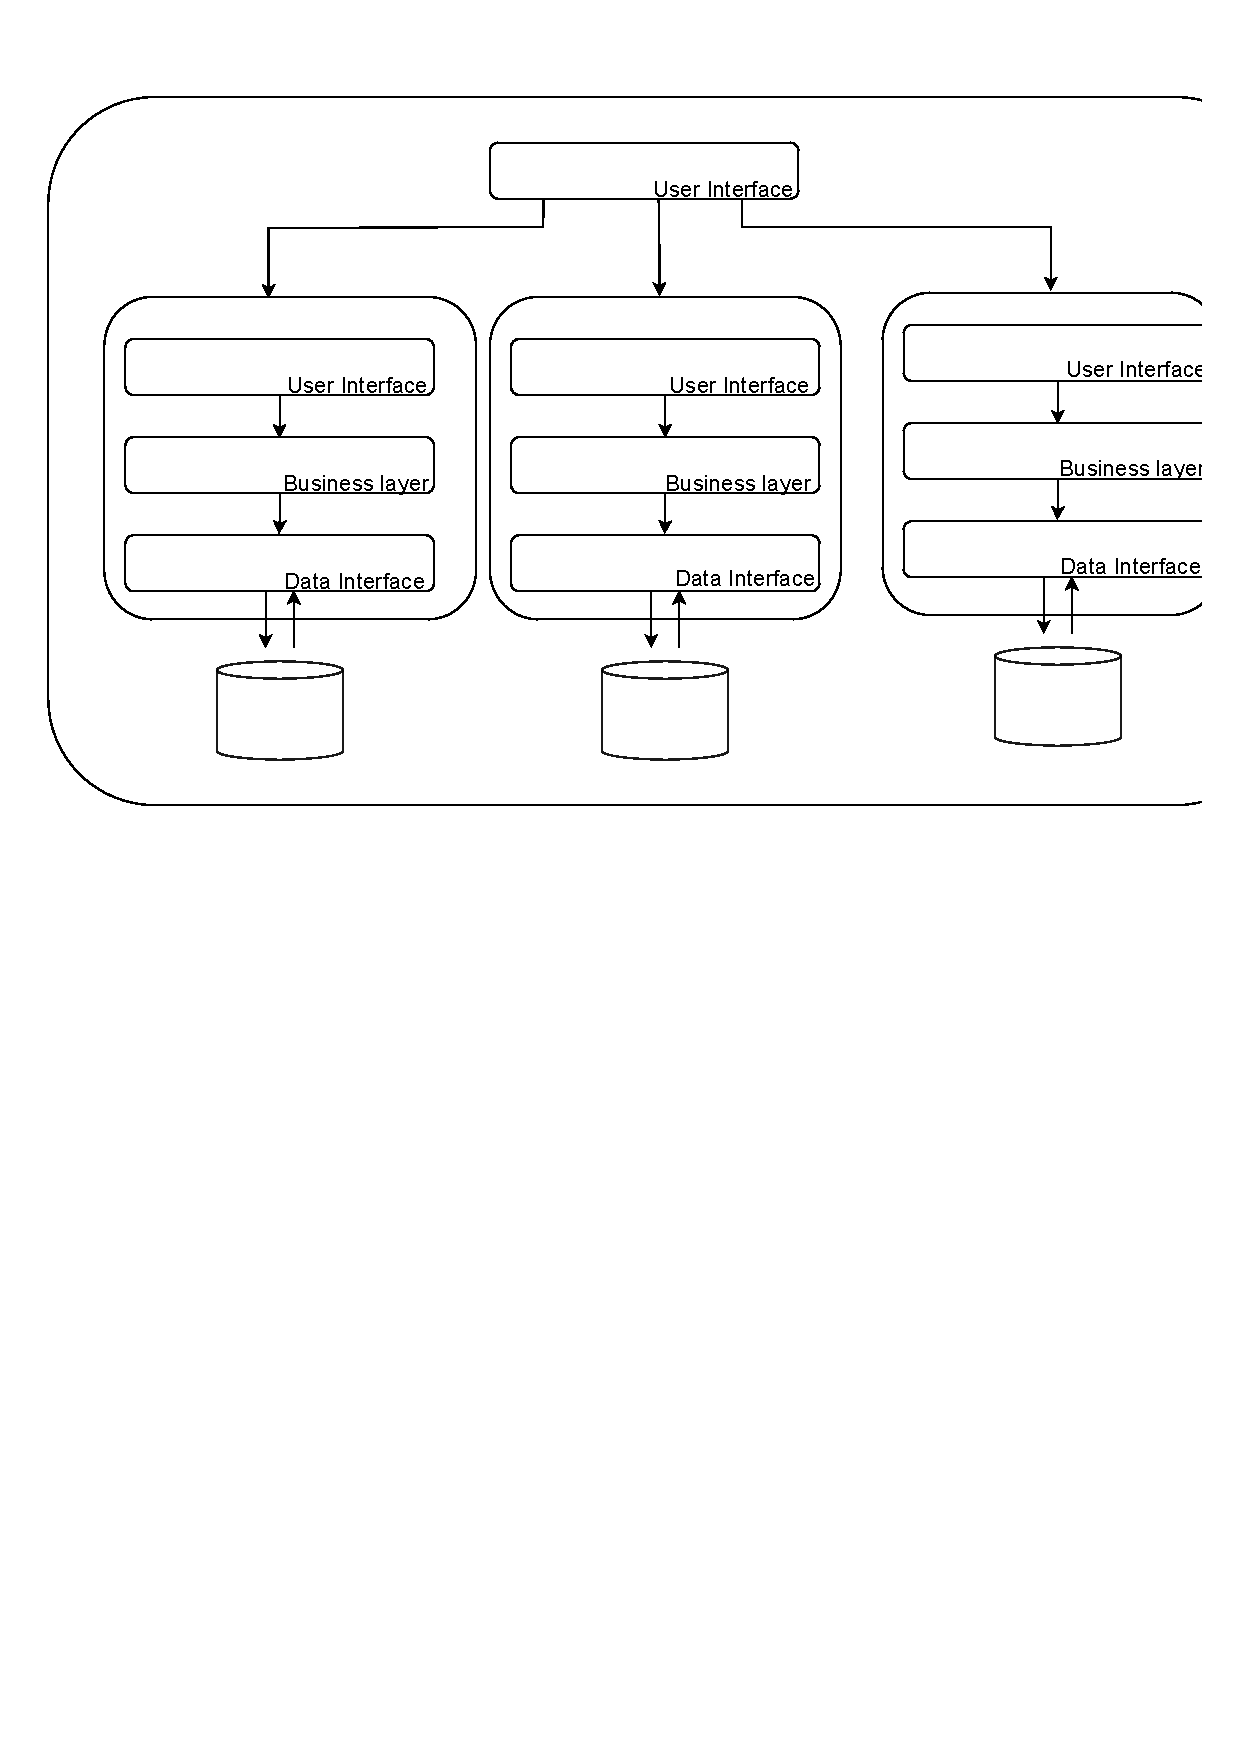
\includegraphics[scale=0.55]{imglib/mono/modular-mono}
        \caption{Aufbau einer Modulare monolitische Architektur}
        \label{fig:microkernel}
    \end{figure}
\end{frame}
\begin{frame}{Modular monolith Architecture: Beispiel E-Commerce I}
    \begin{itemize}
        \item Der OrderService erstellt und speichert die Bestellung mithilfe des OrderRepository
        \item Der OrderService verarbeitet die Zahlung, indem er den PaymentService aufruft
        \item Der OrderService kümmert sich um den Versand, indem er den ShipmentService aufruft.
      \end{itemize}
\end{frame}

\begin{frame}{Monolith Architecture: Beispiel E-Commerce II}
    \begin{figure}[!h]
        \centering
        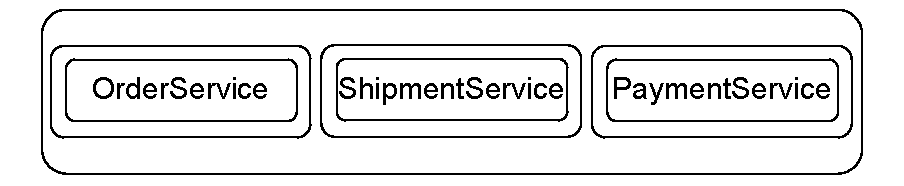
\includegraphics[scale=0.55]{imglib/mono/mono-example}
        \caption{E-Commerce-Beispiel mit Monolith Architektur}
        \label{fig:microkernel-ecommerce}
    \end{figure}
\end{frame}

\begin{frame}{Monotlith Architecture und Modulare monolithische Architecture: Agilität}
    \begin{itemize}
      \item Wiederverwendung in Monolithen nicht vorhanden
    \end{itemize}
\end{frame}


